\chapter{HASIL DAN PEMBAHASAN}

\section{Persiapan Pengujian}
Pengujian hasil penelitian dibagi menjadi tiga kategori, yaitu pengujian daya rendah, pengujian \textit{rapid static survey}, dan pengujian bergerak. Pada pengujian daya rendah dan pengujian \textit{rapid static survey} hanya akan ditinjau dari sisi modul Teseo-LIV3FL saja, sedangkan pada pengujian bergerak akan ditinjau juga dari sisi mikrokontroler.

Sebelum dilakukan pengujian akan dilakukan konfigurasi terhadap modul Teseo-LIV3FL terlebih dahulu. Konfigurasi yang dilakukan ialah untuk mengatur daftar konstelasi yang akan digunakan oleh modul Teseo-LIV3FL. Konstelasi yang akan digunakan adalah GPS, BeiDou, Galileo, dan QZSS.

Pengaturan dilakukan dengan cara mengirimkan perintah untuk mengatur parameter \textit{Configuration Data Blocks} atau CBD pada CBD-ID 200 dan CBD-ID 227. CDB-ID 200 dan CDB-ID 227 digunakan untuk mengaktifkan dan menonaktifkan fitur pada modul Teseo-LIV3FL. Setiap fitur dipetakan pada peta 64-bit dengan CDB-ID 200 merepresentasikan 32-bit pertama dan CDB-ID 227 merepresentasikan 32-bit terakhir. Adapun perintah yang dikirimkan ke modul Teseo-LIV3FL adalah sebagai berikut: 

\begin{verbatim}
	$PSTMSETPAR, 1200, E70000
	$PSTMSETPAR, 1227, 3C0
	$PSTMSETPAR, 1227, C0
	$PSTMSAVEPAR
	$PSTMSSR
\end{verbatim}

Setiap hasil pengujian akan direkam dengan menggunakan aplikasi CoolTerm yang berperan sebagai \textit{serial monitor}. Pada pengujian daya rendah dan pengujian \textit{rapid static survey} akan digunakan perangkat USB \textit{to} TTL \textit{converter} untuk membaca keluaran berupa kalimat NMEA dari modul Teseo-LIV3FL.

\section{Pengujian Daya Rendah}
Pada pengujian daya rendah, modul Teseo-LIV3FL dan multimeter akan dirangkai dengan konfigurasi \textit{common ground}. Perangkat USB \textit{to} TTL \textit{converter} digunakan untuk menghubungkan modul Teseo-LIV3FL dengan komputer sekaligus sebagai sumber arus untuk menyalakan modul Teseo-LIV3FL. Gambar \ref{Fig: low-power-connected} menunjukan modul Teseo-LIV3FL yang sudah terhubung dengan multimeter.

\begin{figure}[H]
	\centering
	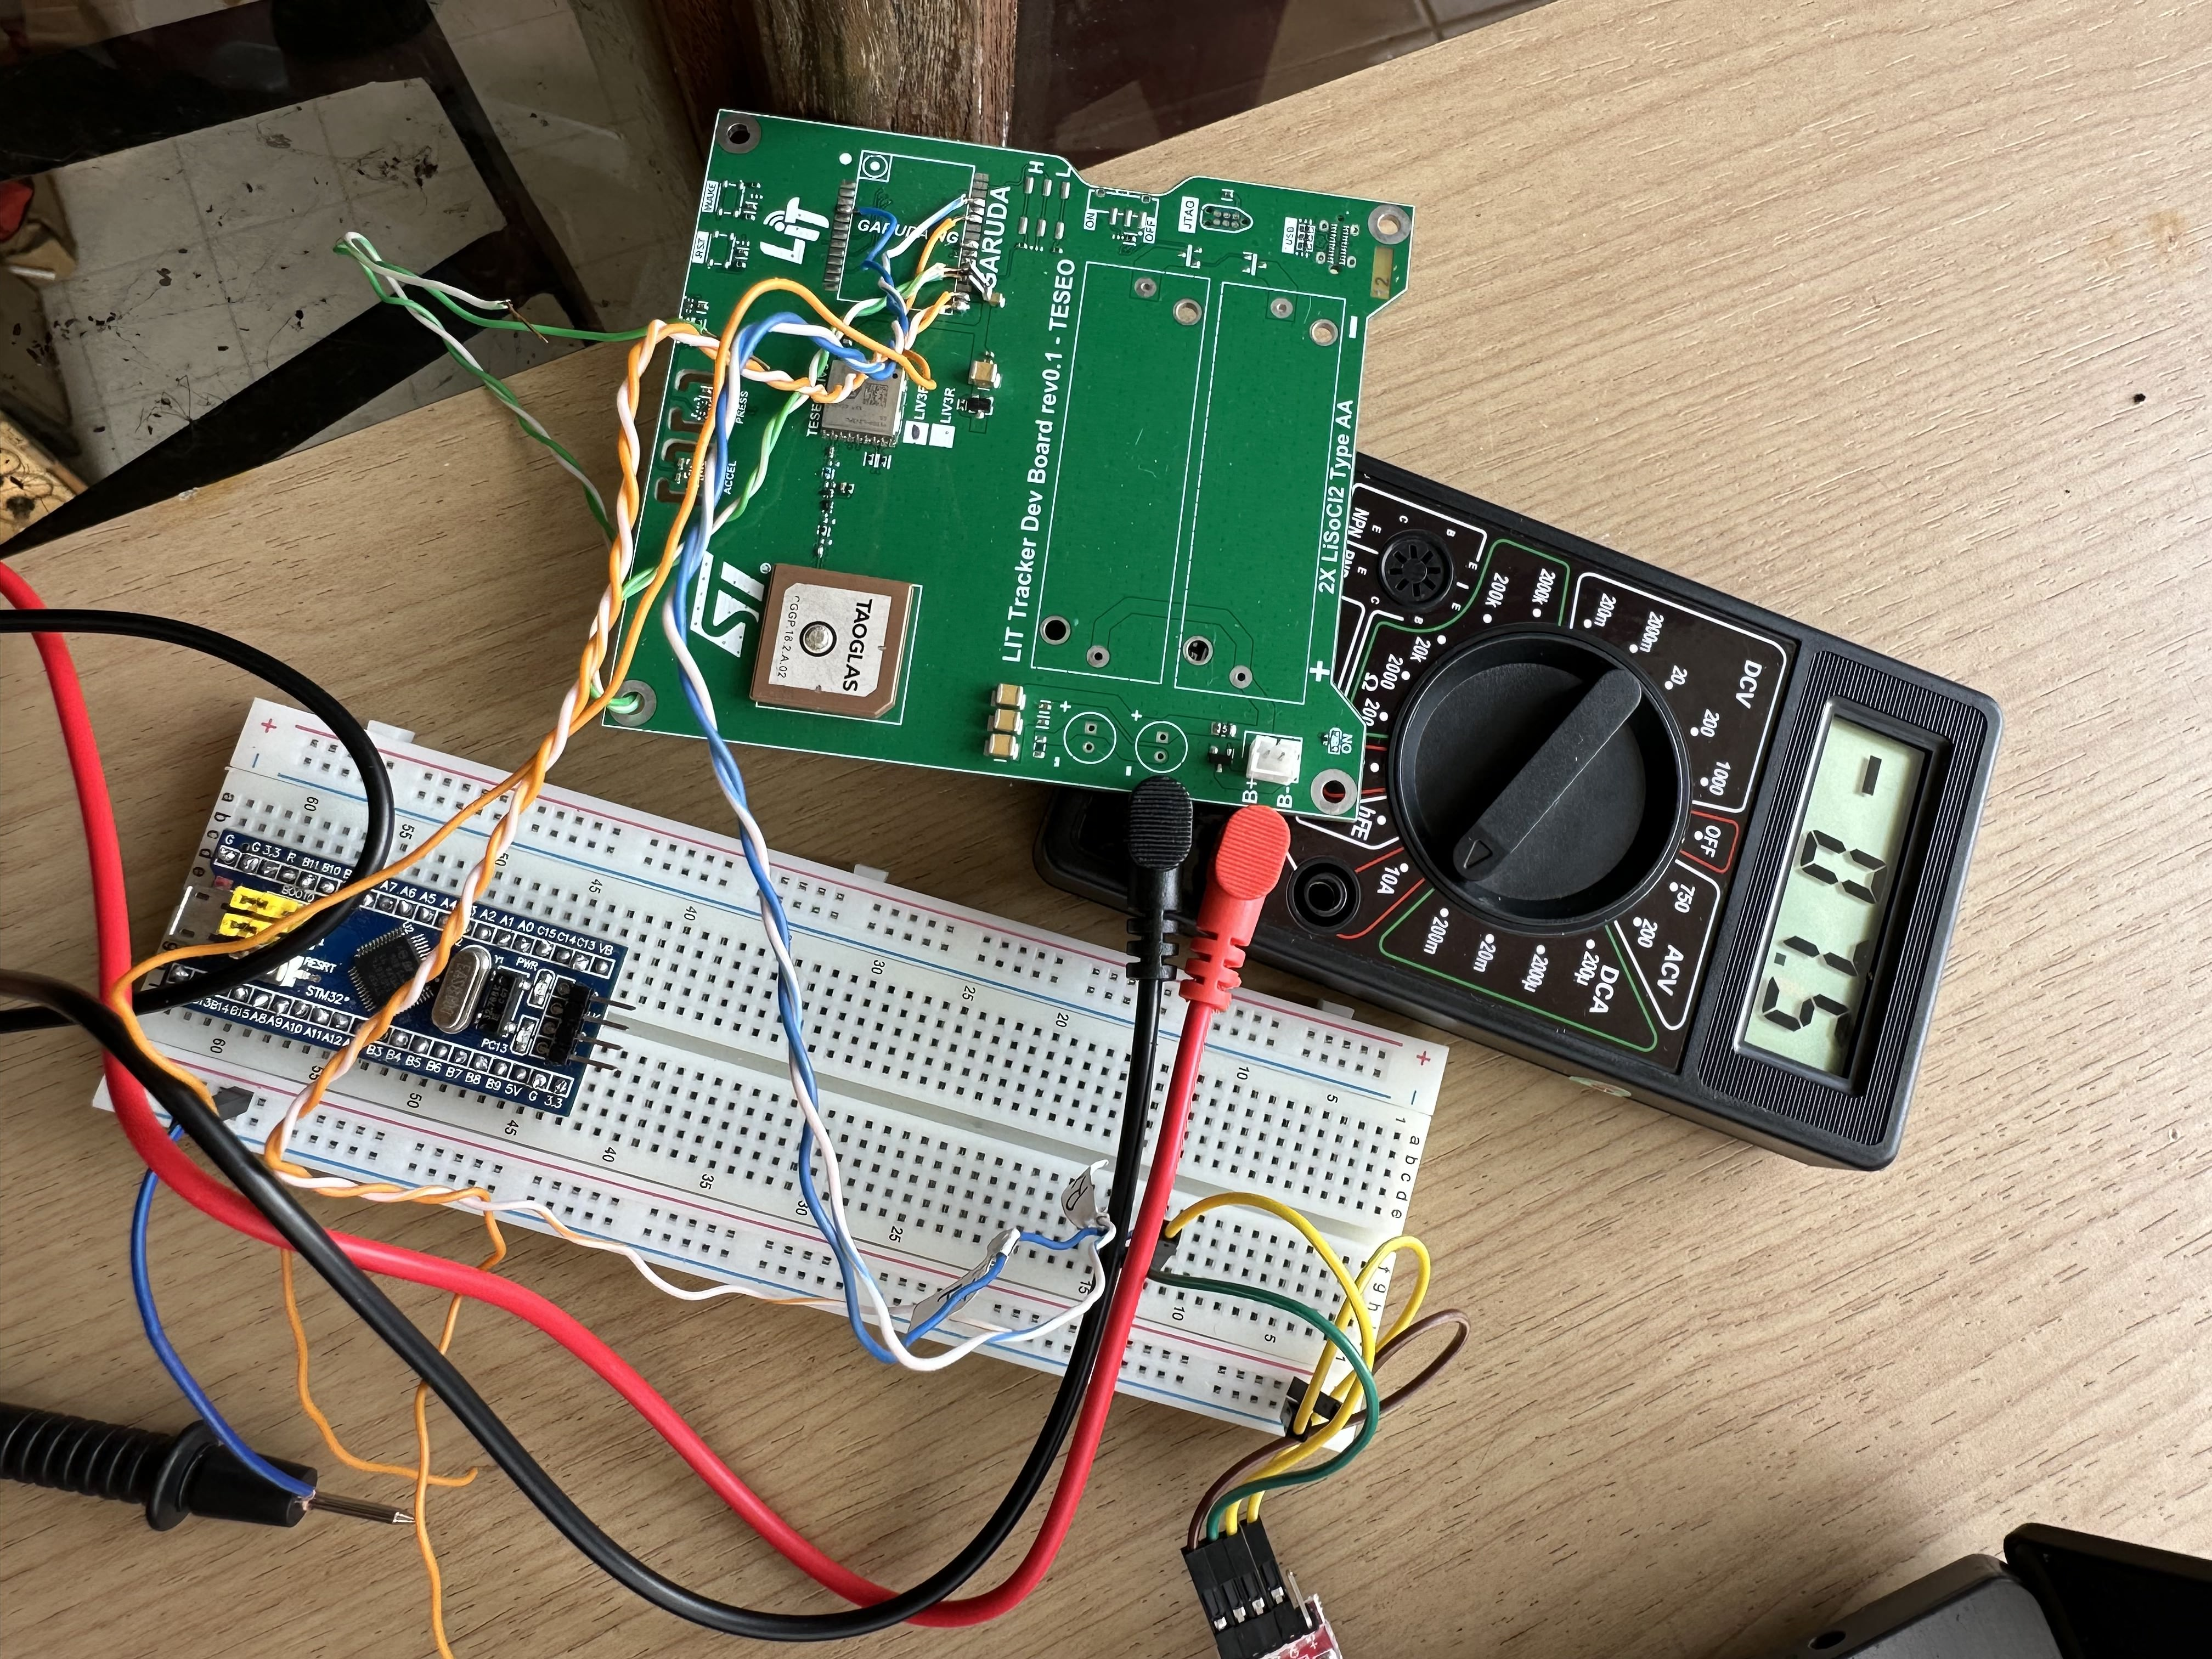
\includegraphics[width=10cm]{contents/chapter-4/low-power.jpg}
	\caption{Modul GNSS yang telah Terangkai dengan Multimeter}
	\label{Fig: low-power-connected}
\end{figure}

Algoritma daya rendah yang digunakan pada pengujian ini adalah mode periodik. Pada mode periodik modul Teseo-LIV3FL akan berada dalam mode akuisisi dalam waktu tertentu hingga mendapat posisi \textit{fix}. Ketika sudah mendapatkan posisis \textit{fix} maka modul Teseo-LIV3FL akan menuju mode \textit{stand by} dan akan menuju dalam mode akuisisi kembali setelah waktu tertentu. Jika modul Teseo-LIV3FL tidak bisa mendapatkan posisi \textit{fix} maka ia juga akan menuju mode \textit{stand by} dan akan mencoba mendapatkan \textit{fix} kembali setelah periode waktu tertentu.

\begin{figure}[H]
	\centering
	\captionsetup{justification=centering}
	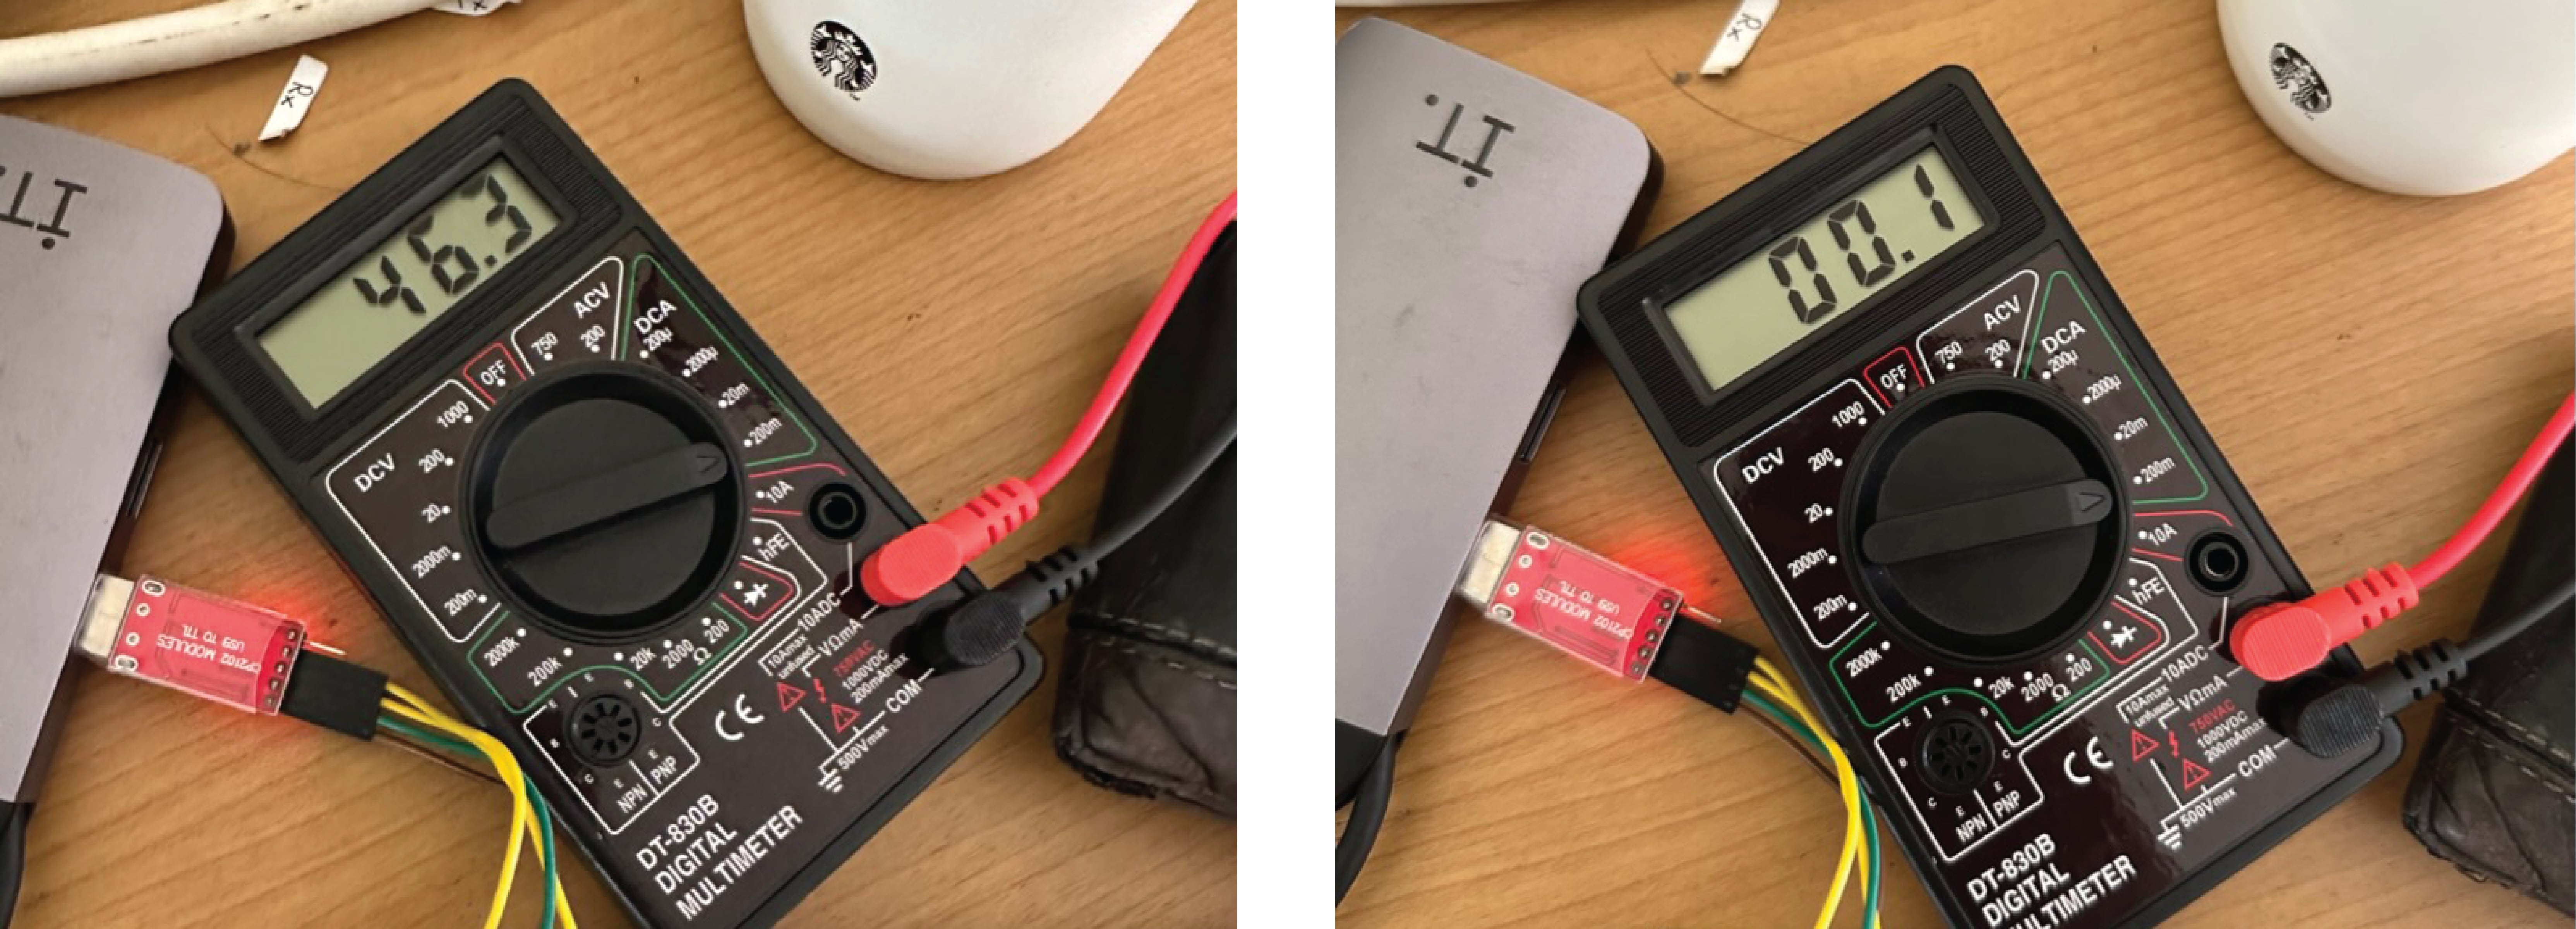
\includegraphics[width=14cm]{contents/chapter-4/low-power-result.jpg}
	\caption{Pembacaan Multimeter pada Mode Akuisisi (Kiri) dan Mode \textit{Stand By} (Kanan)}
	\label{Fig: low-power-result}
\end{figure}

Untuk menyalakan mode daya rendah dapat dilakukan dengan mengirimkan perintah \$PSTMLOWPOWERONOFF. Perintah \$PSTMLOWPOWERONOFF menerima empat belas argumen dengan argumen kedua s.d. kelima untuk mode adaptif, dua argumen selanjutnya untuk mode \textit{cyclic}, dan delapan argumen terakhir untuk mode periodik. Karena digunakan mode periodik maka argumen kedua sampai dengan ketujuh harus diisi dengan angka nol. Perintah yang dikirimkan pada pengujian ini adalah sebagai berikut

\begin{verbatim}
	$PSTMLOWPOWERONOFF,1,0,0,0,0,0,0,3,60,1,1,1,60,30
\end{verbatim}

Perintah di atas akan mengaktifkan mode daya rendah periodik dengan waktu \textit{stand by} selama satu menit setelah mendapatkan tiga posisi \textit{fix}. Selain itu, modul Teseo-LIV3FL akan menuju mode \textit{stand by} selama tiga puluh detik jika tidak dapat mendapatkan posisi \textit{fix} selama satu menit. Detail argumen pada pengujian ini dijelaskan pada Tabel 4.1.

\begin{longtblr}[caption = {Argumen pada Perintah \$PSTMLOWPOWERONOFF}]{
		width = \linewidth,
		colspec = {Q[285]Q[48]Q[608]},
		row{1} = {c},
		row{3} = {c},
		row{5} = {c},
		row{6} = {c},
		row{7} = {c},
		row{8} = {c},
		row{10} = {c},
		row{11} = {c},
		cell{2}{1} = {c},
		cell{2}{2} = {c},
		cell{3}{1} = {c=3}{0.941\linewidth},
		cell{4}{1} = {c},
		cell{4}{2} = {r=4}{c},
		cell{4}{3} = {r=4}{},
		cell{8}{1} = {c=3}{0.941\linewidth},
		cell{9}{1} = {c},
		cell{9}{2} = {r=2}{c},
		cell{9}{3} = {r=2}{},
		cell{11}{1} = {c=3}{0.941\linewidth},
		cell{12}{1} = {c},
		cell{12}{2} = {c},
		cell{13}{1} = {c},
		cell{13}{2} = {c},
		cell{14}{1} = {c},
		cell{14}{2} = {c},
		cell{15}{1} = {c},
		cell{15}{2} = {c},
		cell{16}{1} = {c},
		cell{16}{2} = {c},
		cell{17}{1} = {c},
		cell{17}{2} = {c},
		cell{18}{1} = {c},
		cell{18}{2} = {c},
		hline{1-4,8-9,11-12} = {-}{},
	}
	\label{Tab: pstmlponoff-result}
	\textbf{Argumen}                               & \textbf{Nilai} & \textbf{Keterangan}                                                                                                                      \\
	Menyalakan atau mematikan mode daya rendah     & 1              & Mode daya rendah dinyalakan                                                                                                              \\
	Mode Adaptif                                   &                &                                                                                                                                          \\
	\textit{Constellation Mask}                    & 0              & Mode adaptif tidak digunakan.                                                                                                            \\
	Batas~\textit{EHPE}                            &                &                                                                                                                                          \\
	Satelit Maksimum                               &                &                                                                                                                                          \\
	Perpindahan Konstelasi Otomatis                &                &                                                                                                                                          \\
	Mode \textit{Cyclic}                           &                &                                                                                                                                          \\
	Menyalakan atau mematiakan \textit{Duty Cycle} & 0              & Mode \textit{cyclic~tidak digunakan.}                                                                                                    \\
	Periode \textit{Duty Cycle}                    &                &                                                                                                                                          \\
	Mode Periodik                                  &                &                                                                                                                                          \\
	Mode Periodik                                  & 3              & Mode periodik \textit{stand by}                                                                                                          \\
	FixPeriod                                      & 60             & Modul akan memasuki mode~\textit{stand by~selama enam puluh detik setelah mendapat posisi \textit{fix}}                                  \\
	FixOnTime                                      & 3              & Memasuki mode \textit{stand by~setelah mendapatkan tiga posisi \textit{fix}}                                                             \\
	Penyegaran Ephemeris                           & 1              & Penyegaran ephemeris diaktifkan                                                                                                          \\
	Kalibrasi RTC                                  & 1              & Kalibrasi RTC diaktifkan                                                                                                                 \\
	NoFixCnt                                       & 60             & Modul akan memasuki mode \textit{stand by~jika tidak bisa mendapatkan posisi \textit{fix~setelah enam puluh detik (\textit{fix lloss)}}} \\
	NoFixOff                                       & 30             & Modul memasuki \textit{stand by~selama tiga puluh detik setelah \textit{fix loss.}}                                                      
\end{longtblr}

Dalam mode akuisisi, arus yang mengalir pada modul Teseo-LIV3FL adalah sebesar 46.3 mA atau  18,7 mA lebih kecil jika dibandingkan dengan \textit{datasheet}. Pada mode \textit{stand by}, arus yang mengalir pada modul Teseo-LIV3FL sudah mendekati \textit{datasheet} (10$\mu$A), yaitu sebesar 15 $\mu$A. Gambar \ref{Fig: low-power-result} sebelah kiri menunjukan hasil pengukuran multimeter ketika modul Teseo-LIV3FL berada dalam mode akuisisi dan sebelah kanan ketika modul Teseo-LIV3FL berada dalam mode \textit{stand by}.

\section{Pengujian \textit{Rapid Static Survey}}
Rapid Static Survey adalah pengujian yang dilakukan untuk meninjau performa modul GNSS dalam keadaan diam. Pengujian ini dapat dilakukan dalam rentang waktu lima belas menit s.d. dua jam (Lauer, 2018). Pengujian ini akan meninjau akurasi dan presisi dari modul GNSS. Akurasi adalah tingkat kedekatan hasil pembacaan modul GNSS dengan posisi sebenarnya, sedangkan tingkat presisi menunjukan seberapa dekat hasil yang didapat dengan rata-rata dari seluruh sampel (Novatel, 2003).

Pada pengujian rapid static survey, modul Teseo-LIV3FL diletakan dalam empat skenario selama satu jam. Skenario tersebut meliputi \textit{basemet}, dalam ruangan, ruangan semi terbuka, dan ruang terbuka. Pengujian setiap skenario dilakukan pada empat titik di lingkungan Universitas Gadjah Mada, yaitu:
\begin{enumerate}
	\item \textit{Basement} diwakili oleh tempat parkir bawah tanah milik Fakultas Ilmu Sosial dan Ilmu Politik.
	\item Ruangan tertutup diwakili oleh Lantai 5 Gedung SGLC Fakultas Teknik
	\item Ruang semi terbuka diwakili oleh Selasar Grha Sabha Pramana.
	\item Ruangan terbuka diwakili oleh Lapangan Pancasila
\end{enumerate}

Modul Teseo-LIV3FL dihubungkan dengan protokol komunikasi UART pada baud rate 115.200 Bps menggunakan konversi USB to TTL. Pengujian ini akan meninjau nilai HDOP, VDOP, PDOP, dan CEP di setiap skenario.

\subsection{Skenario \textit{Basement}}
\begin{table}[H]
	\caption{Hasil Pengujian Skenario \textit{Basement}}
	\vspace{0.5em}
	\centering
	\begin{tabular}{ccccc}
		\hline
		& \textbf{Minima} & \textbf{Maxima} & \textbf{Rata-rata} & \textbf{Standar Deviasi}\\
		\hline 
		HDOP & 1,80 & 26,80 & 8,27 & 5,36\\
		PDOP & 2,80 & 39,30 & 10,67 & 7,30\\
		VDOP & 2,00 & 28,80 & 8,27 & 5,36\\
		CEP & 0 & 79,56 & 32,69 & 13,34\\
		Jumlah Satelit & 5 & 12 & 7,60 & 1,27\\
		\hline
	\end{tabular}
	\label{Tab: basement-table}
\end{table}

Pengujian skenario \textit{basement} dilakukan untuk mengetahui performa modul Teseo-LIV3FL pada ruangan bawah tanah. Modul Teseo-LIV3FL diletakan di tempat parkir bawah tanah milik Fakultas Ilmu Sosial dan Ilmu Politik. Lingkungan pengujian berada di bawah gedung empat lantai dengan struktur beton. Selain itu, terdapat sedikit bagian terbuka yang memungkinkan sinar matahari untuk memasuki ruangan. Gambar \ref{Fig: basement-keadaan} menunjukan kondisi pengujian skenario \textit{basement}.

\begin{figure}[H]
	\centering
	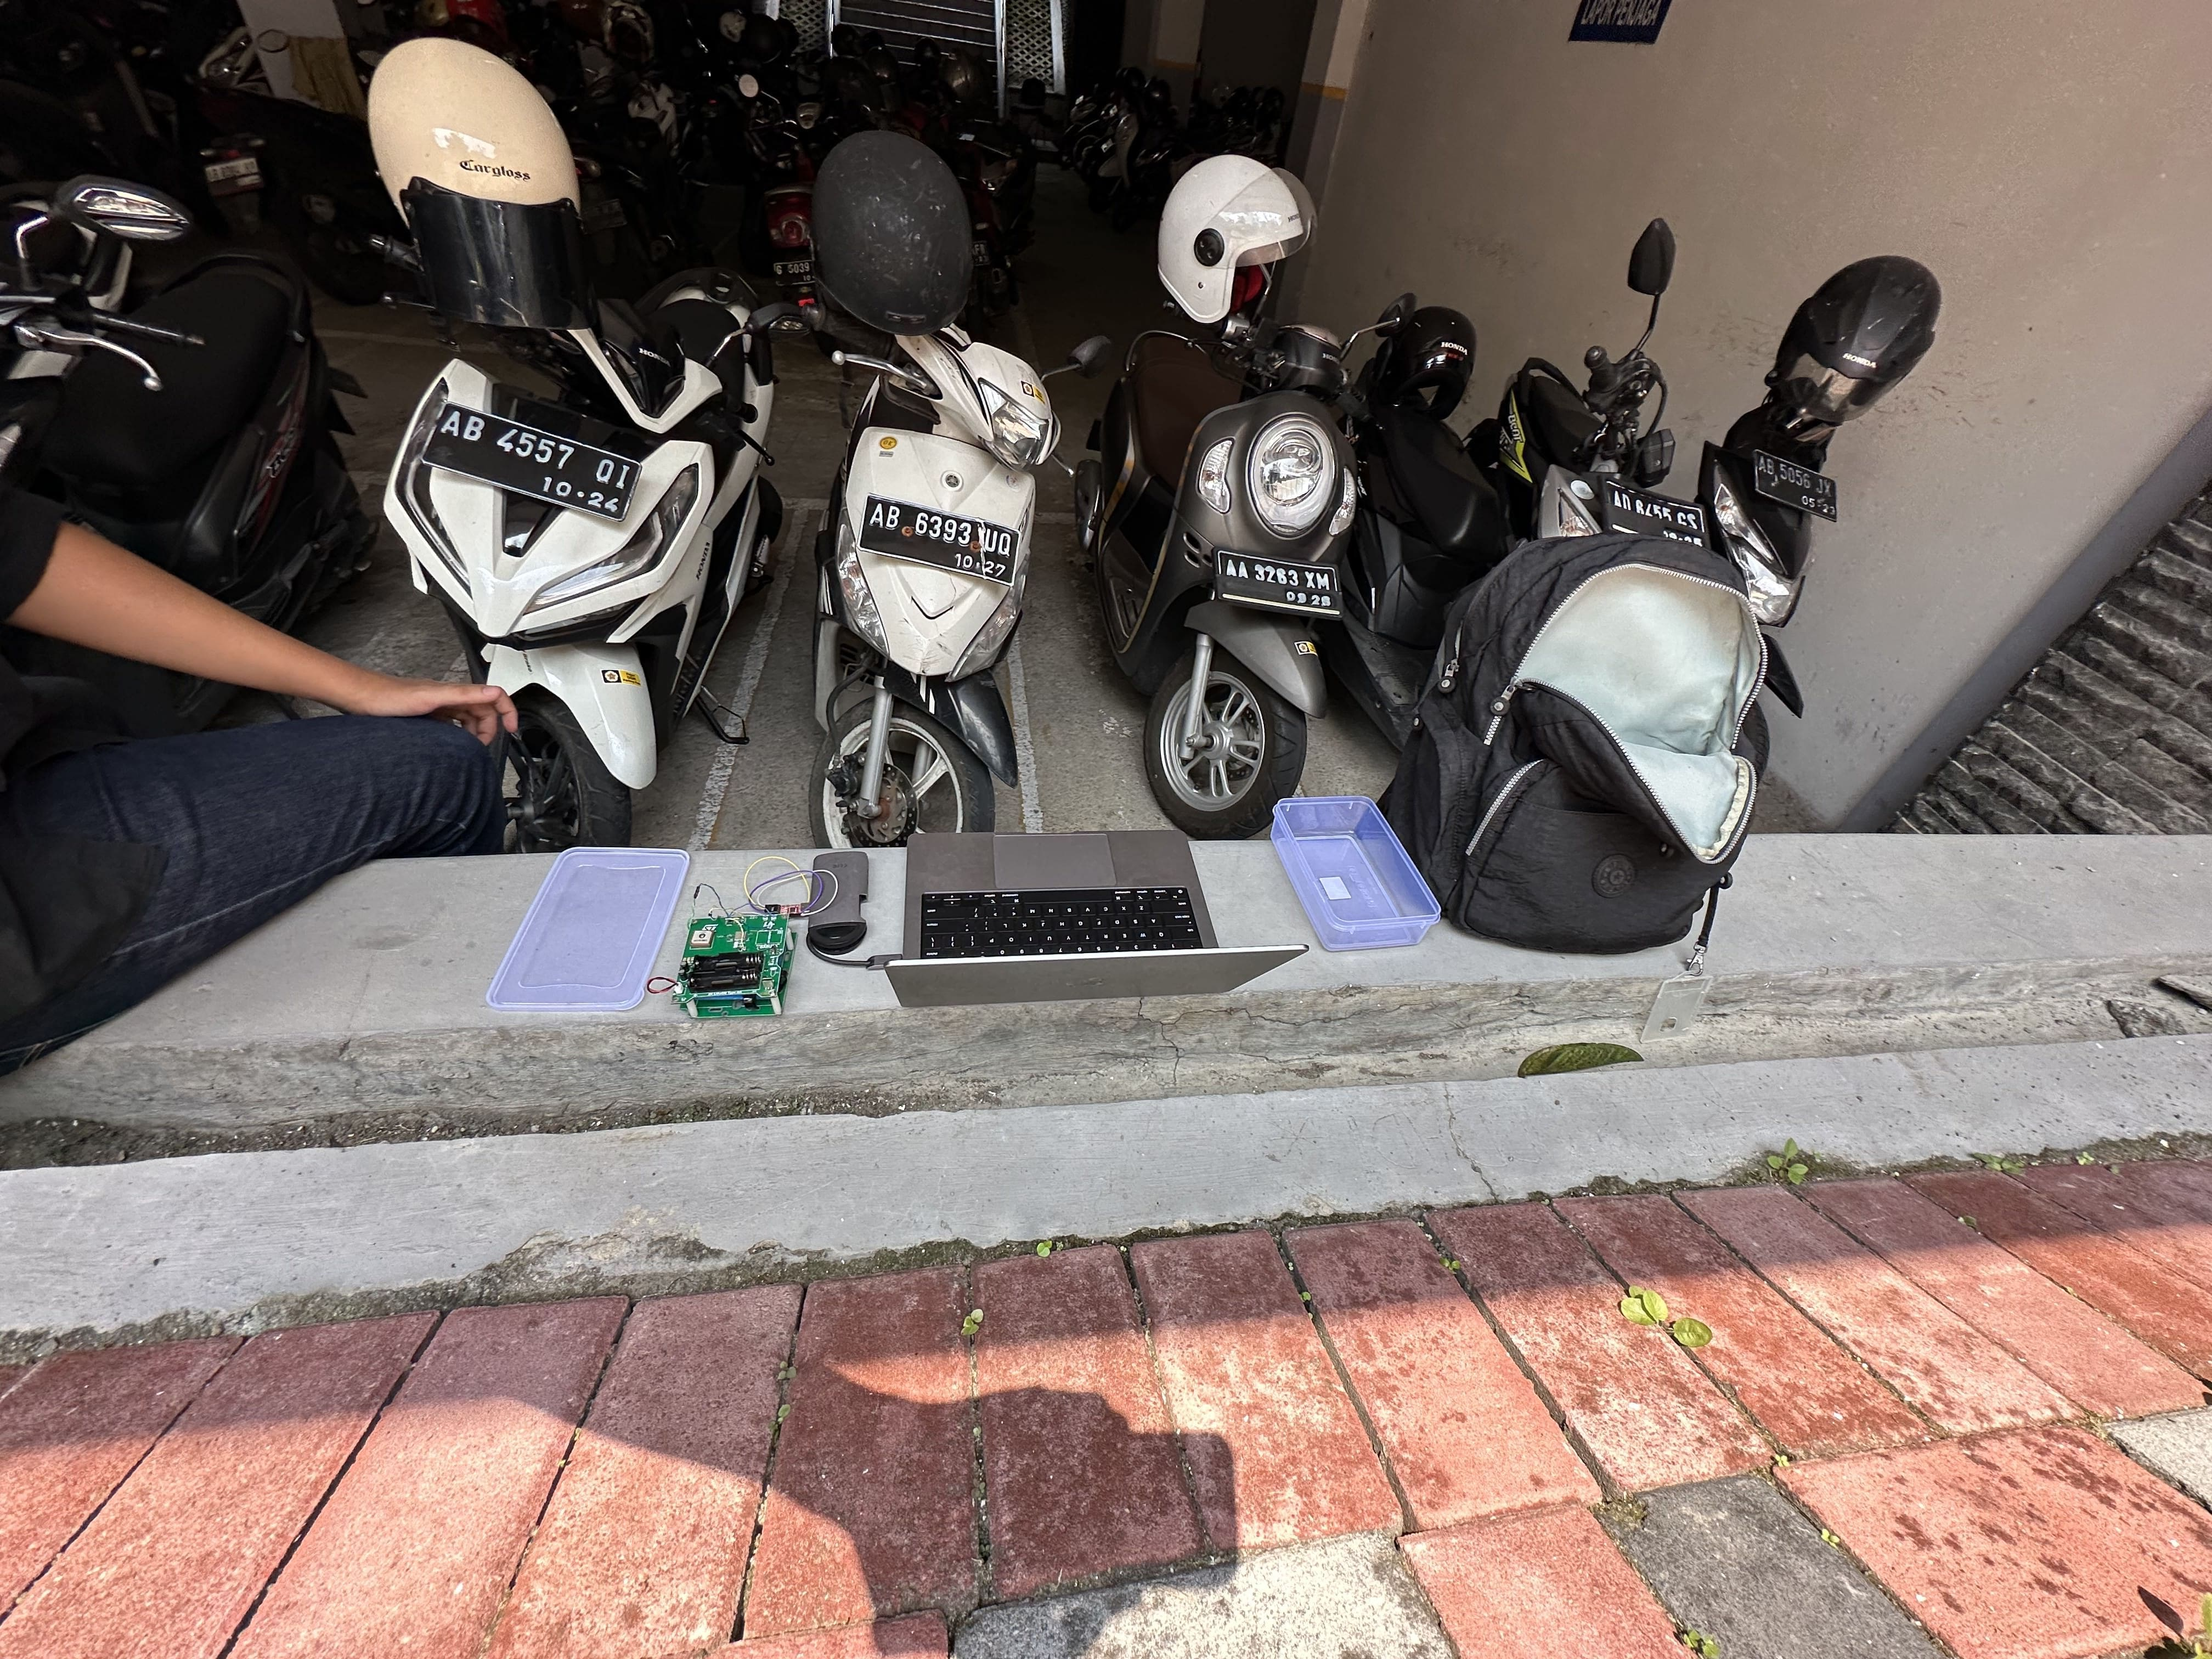
\includegraphics[width=10cm]{contents/chapter-4/1-skenario-basement/keadaan.jpg}
	\caption{Pengujian Skenario \textit{Basement}}
	\label{Fig: basement-keadaan}
\end{figure}

Hasil pembacaan modul Teseo-LIV3FL pada skenario \textit{basement} tidak memberikan hasil yang akurat. Terlihat pada Gambar \ref{Fig: basement-sats_dop} bahwa terjadi lonjakan nilai DOP. Tabel \ref{Tab: basement-table} menunjukan nilai maksimum DOP adalah nilai PDOP sebesar 39,30. Nilai PDOP yang sangat tinggi menunjukan bahwa persebaran satelit di langit tidak mencakup seluruh lingkaran seperti ditunjukan oleh \textit{sky plot} pada Gambar \ref{Fig: basement-skyplot}. \textit{Sky plot} tersebut menunjukan bahwa persebaran satelit hanya mencakup setengah bagian pada lingkaran.

\begin{figure}[H]
	\centering
	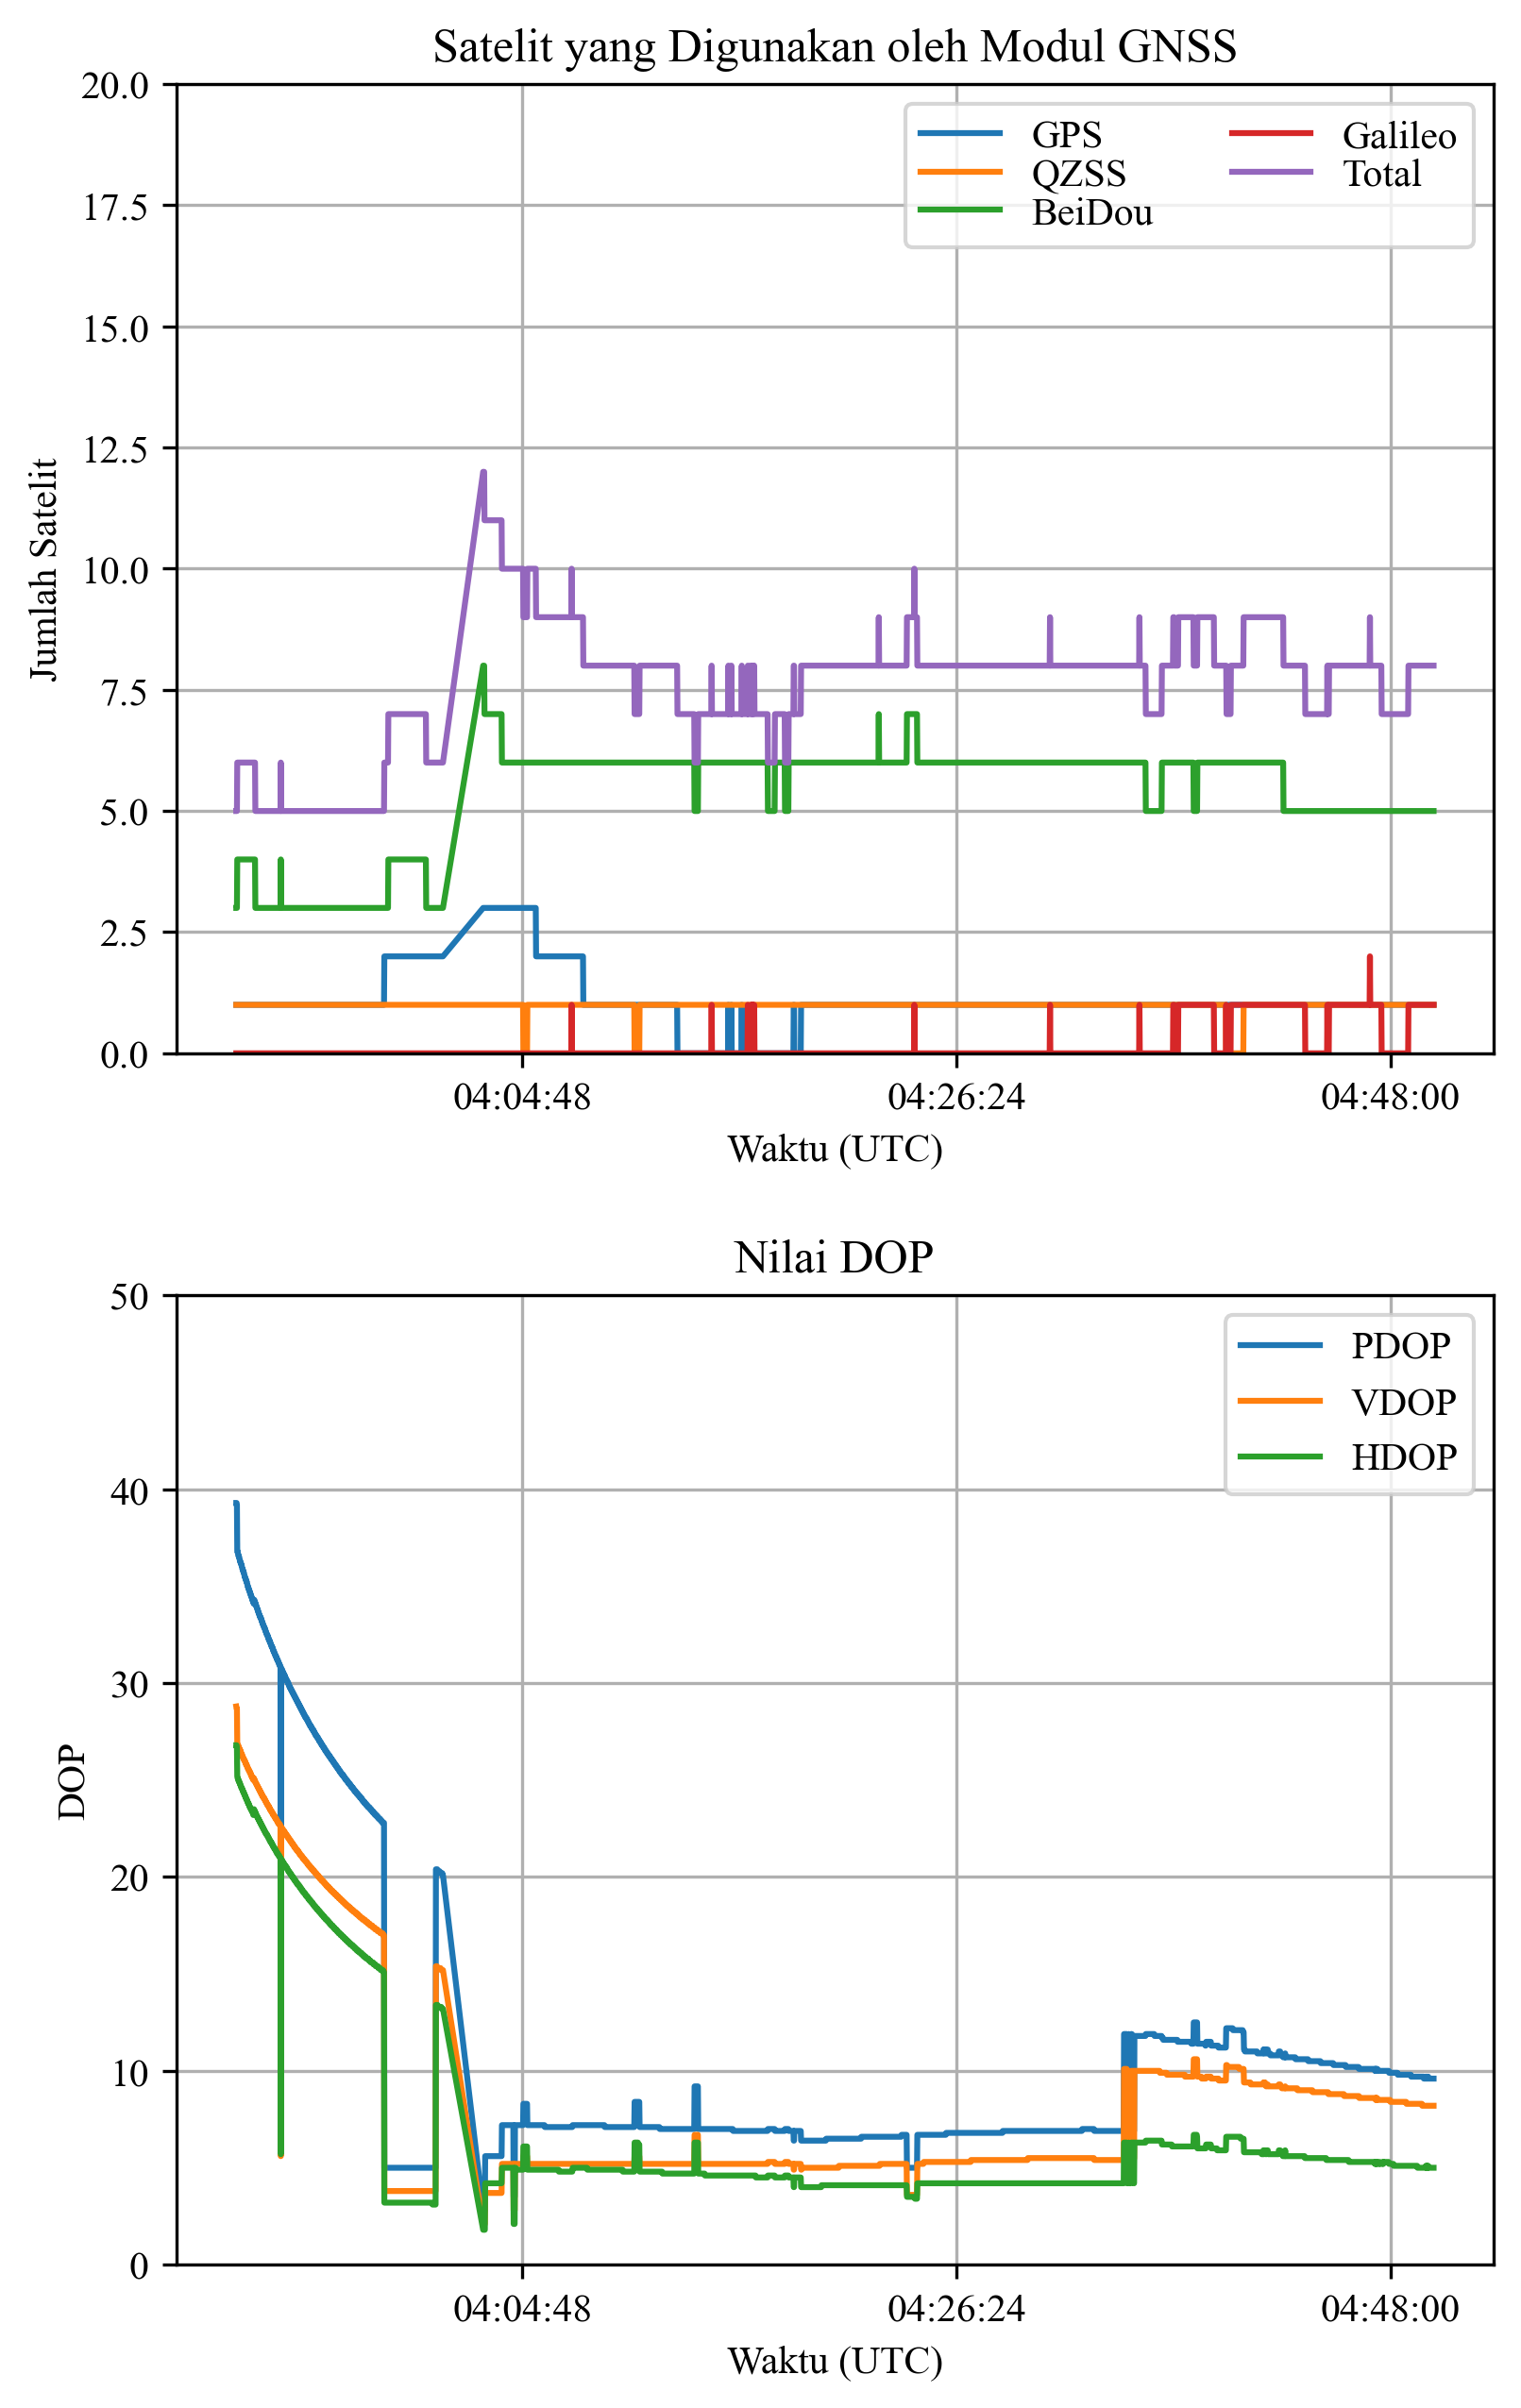
\includegraphics[width=12cm]{contents/chapter-4/1-skenario-basement/sats_dop.png}
	\caption{Jumlah Satelit dan Nilai DOP pada Pengujian Skenario \textit{Basement}}
	\label{Fig: basement-sats_dop}
\end{figure}

Pada skenario \textit{basement}, modul Teseo-LIV3FL tetap dapat menangkap isyarat dari keempat konstelasi Teseo-LIV3FL yang telah diatur meskipun tertutup oleh struktur beton. Konstelasi dengan jumlah satelit adalah BeiDou milik Republik Rakyat Tiongkok. Lonjakan nilai DOP pada awal pengujian terjadi bersamaan dengan keadaan jumlah satelit paling rendah. Hal tersebut menunjukan bahwa jumlah satelit yang rendah akan meningkatkan ketiga nilai DOP yang artinya akan menurunkan akurasi dari hasil pembacaan modul Teseo-LIV3FL.

\begin{figure}[H]
	\centering
	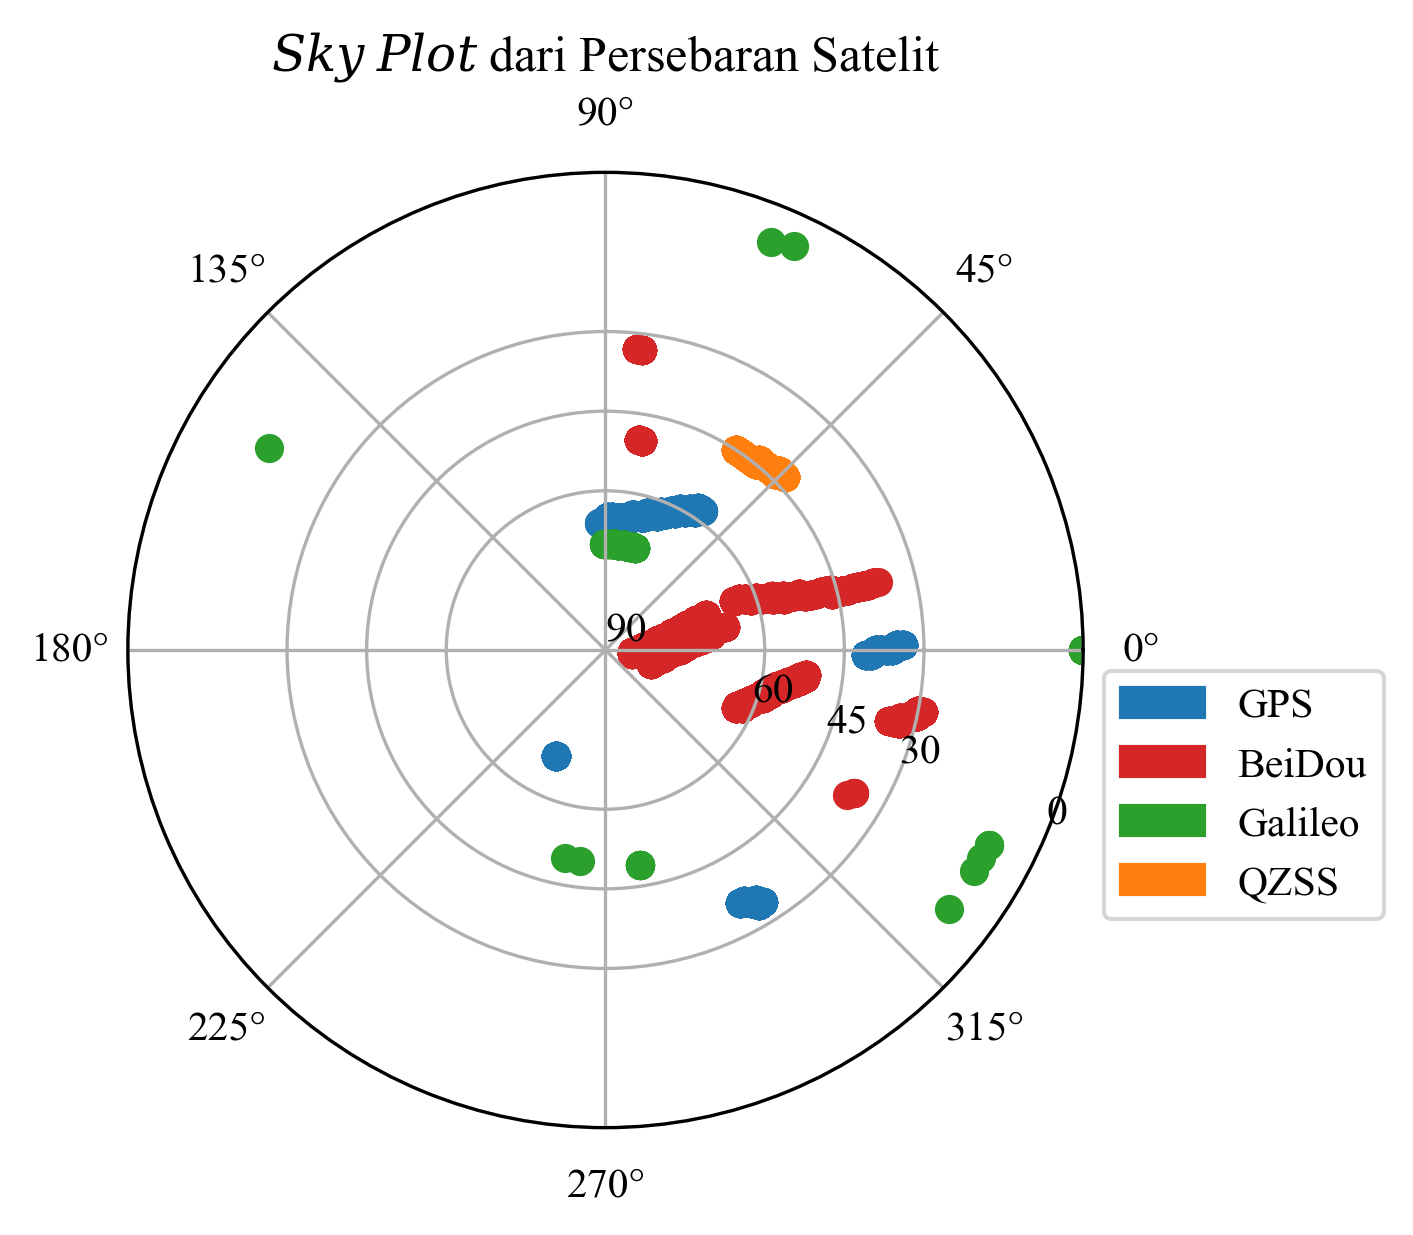
\includegraphics[width=11cm]{contents/chapter-4/1-skenario-basement/skyplot.png}
	\caption{\textit{Sky Plot} Pengujian Skenario \textit{Basement}}
	\label{Fig: basement-skyplot}
\end{figure}

Nilai rata-rata nilai CEP pada pengujian ini adalah 32,69 m yang menunjukan tingkat presisi pada skenario \textit{basement} adalah 32,69 m. Selain itu, rata-rata nilai HDOP pada skenario \textit{basement} menunjukan angka 8,27 yang menunjukan bahwa hasil pengukuran posisi pada skenario ini masih layak untuk digunakan.

Pengujian skenario \textit{basement} menunjukan bahwa modul GNSS masih bisa digunakan dalam ruangan bawah tanah dengan sedikit bagian terbuka. Meskipun mampu untuk mendapatkan posisi \textit{fix}, akurasi yang didapat masih bisa diperbaiki pada skenario selanjutnya.

\subsection{Skenario Dalam Ruangan}
\begin{table}[H]
	\caption{Jenis STM32 dan Arsitekturnya}
	\vspace{0.5em}
	\centering
	\begin{tabular}{ccccc}
		\hline
		& \textbf{Minima} & \textbf{Maxima} & \textbf{Rata-rata} & \textbf{Standar Deviasi}\\
		\hline 
		HDOP & 1,30 & 6,80 & 2,79 & 0,68\\
		PDOP & 2,00 & 8,40 & 3,73 & 0,74\\
		VDOP & 1,40 & 5,50 & 2,48 & 0,94\\
		CEP & 9,51	& 33,27 & 12,14 & 4,02\\
		Jumlah Satelit & 8 & 15 & 10,93 & 1,14\\
		\hline
	\end{tabular}
	\label{Tab: indoor-table}
\end{table}

Pengujian skenario dalam ruangan dilakukan untuk meninjau performa modul Teseo-LIV3FL di dalam ruangan tertutup. Titik pengujian berada di lantai 5 Gedung SGLC Fakultas Teknik. Lingkungan sekitar pengujian merupakan suatu ruangan dengan jendela besar yang memungkinkan lebih banyak sinar matahari untuk memasuki ruangan. Gambar \ref{Fig: indoor-keadaan} menunjukan pengujian skenario dalam ruangan.

\begin{figure}[ht]
	\centering
	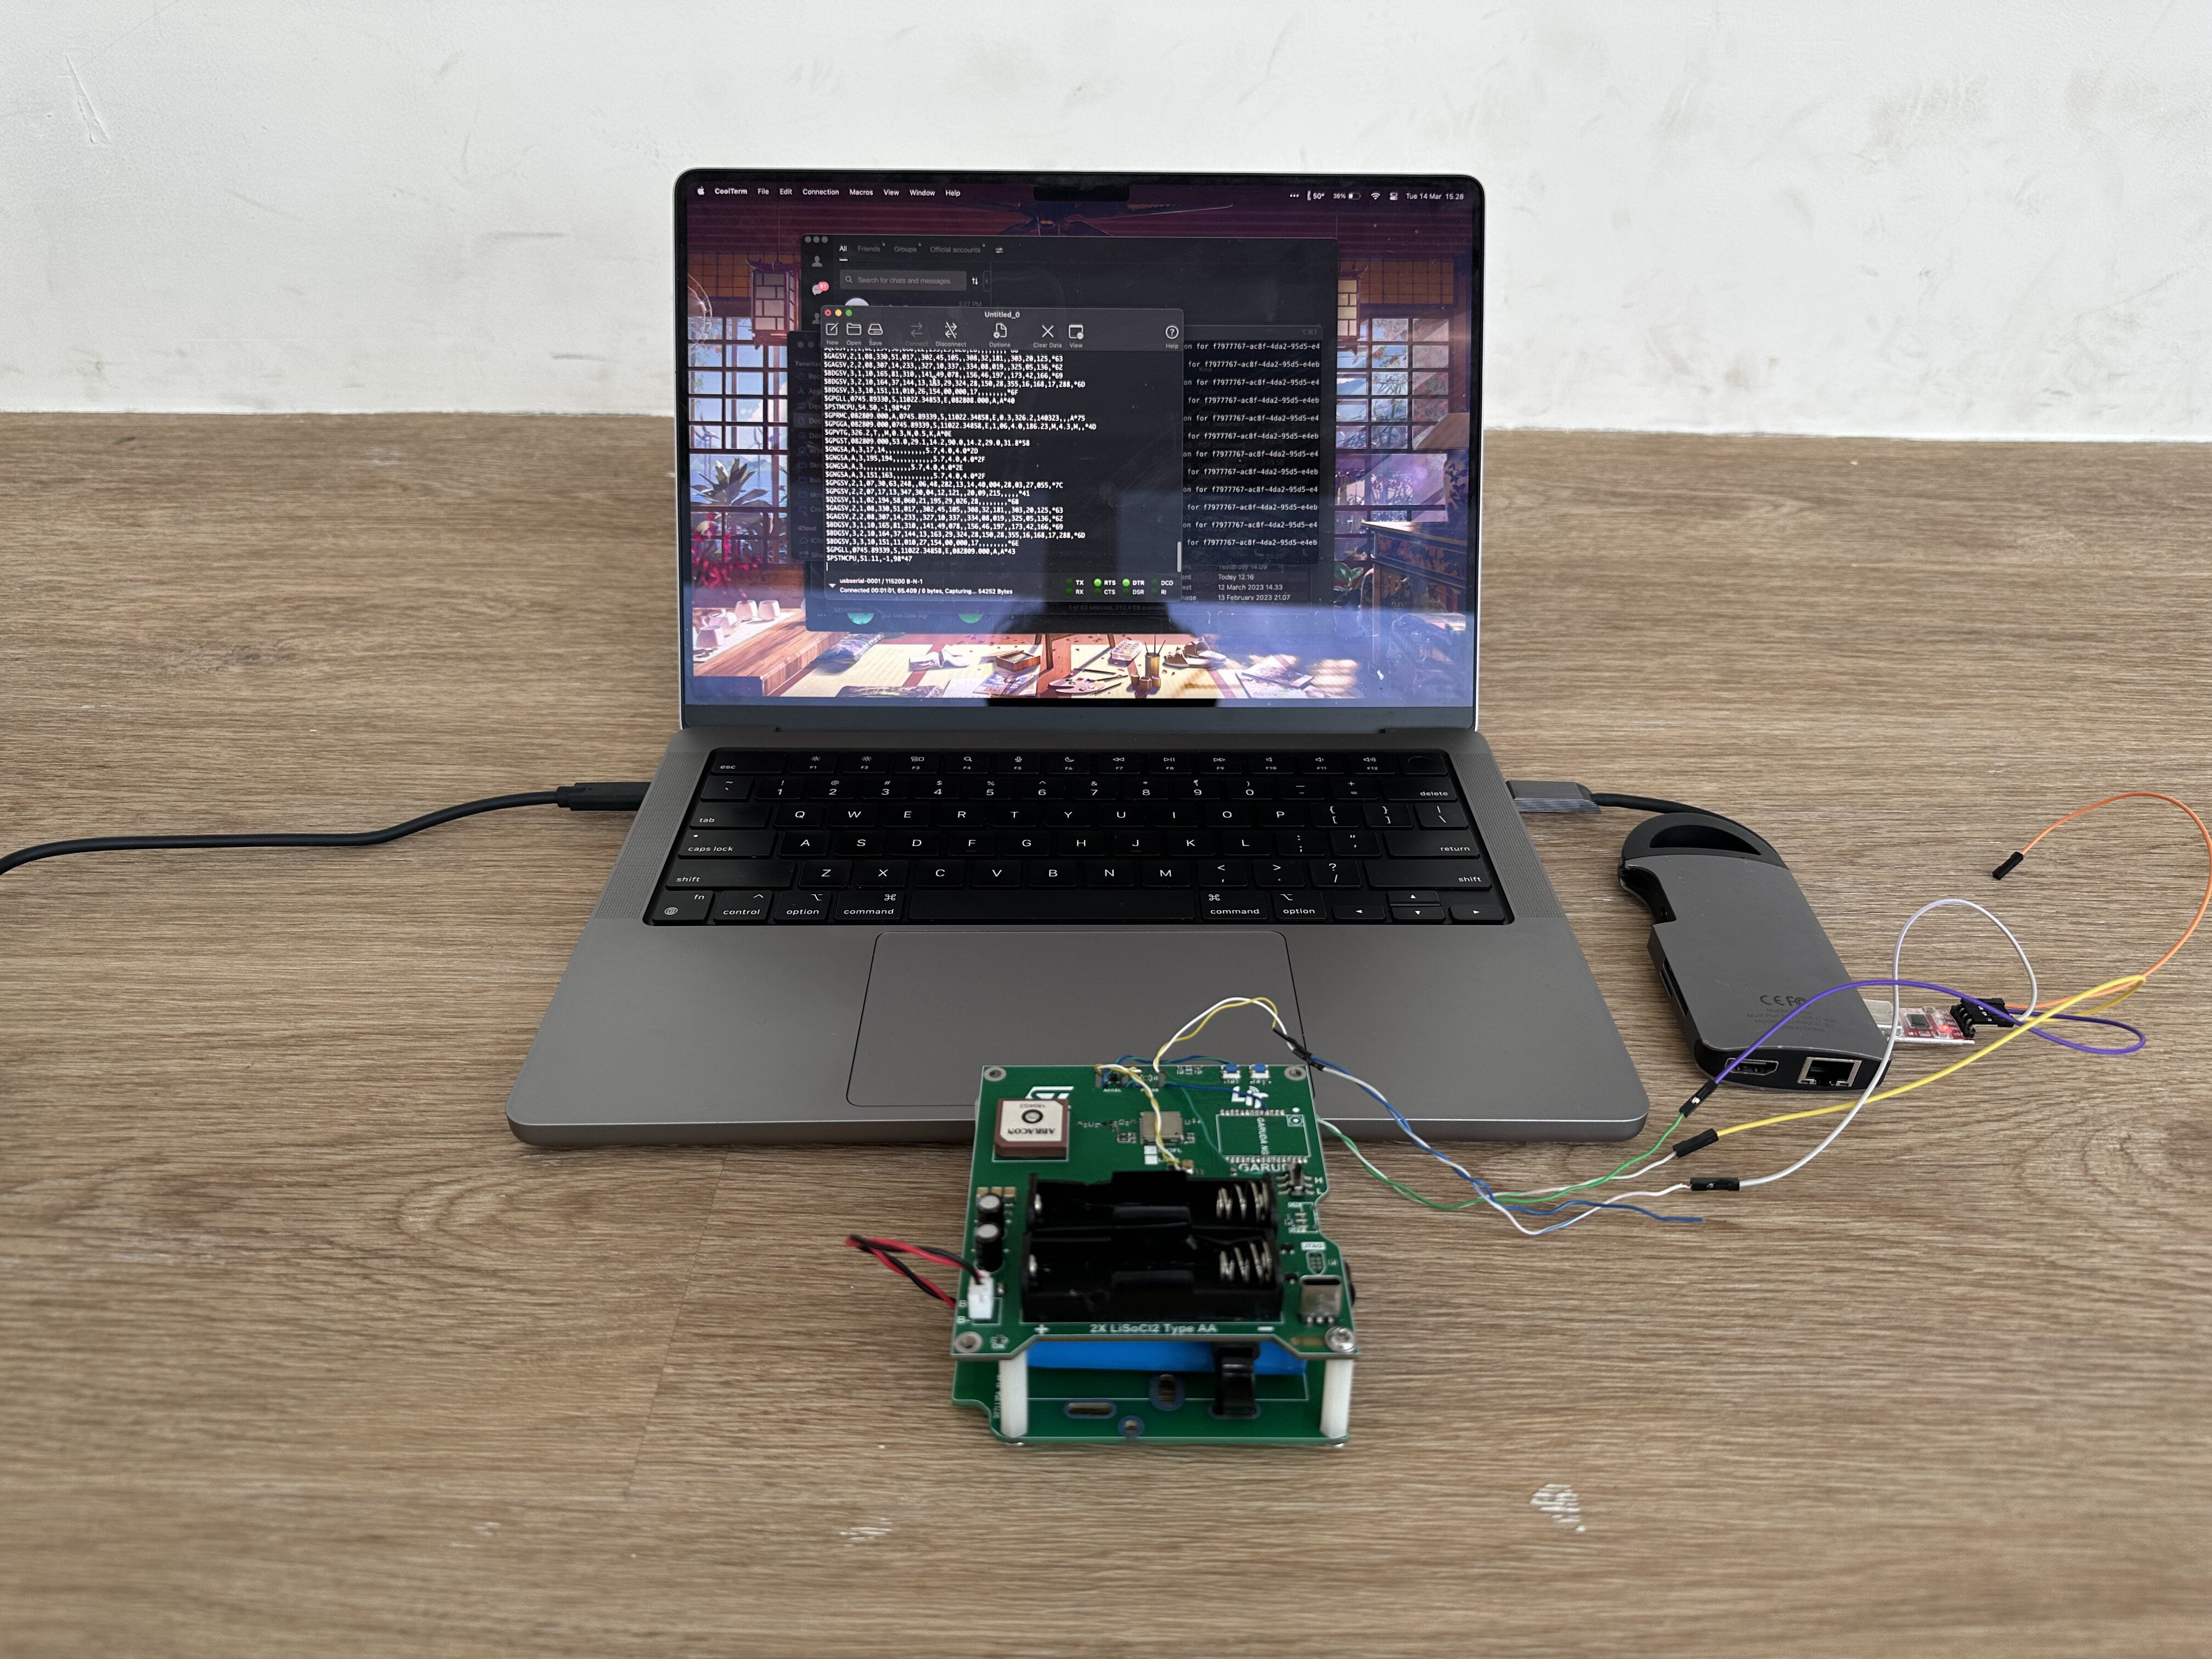
\includegraphics[width=10cm]{contents/chapter-4/2-skenario-indoor/keadaan.jpg}
	\caption{Pengujian Skenario Dalam Ruangan}
	\label{Fig: indoor-keadaan}
\end{figure}

Sama seperti pada pengujian skenario \textit{basement}, modul Teseo-LIV3FL juga dapat menerima isyarat dari keempat konstelasi yang telah diatur sebelumnya seperti ditunjukan pada Gambar \ref{Fig: indoor-sats_dop}. Konstelasi dengan jumlah satelit paling banyak adalah BeiDou dan GPSS. Jumlah satelit pada konstelasi QZSS hampir selalu konstan pada sebanyak dua buah, sedangkan konstelasi Galileo bervariasi antara nol s.d. empat buah satelit.

\begin{figure}[H]
	\centering
	\captionsetup{justification=centering}
	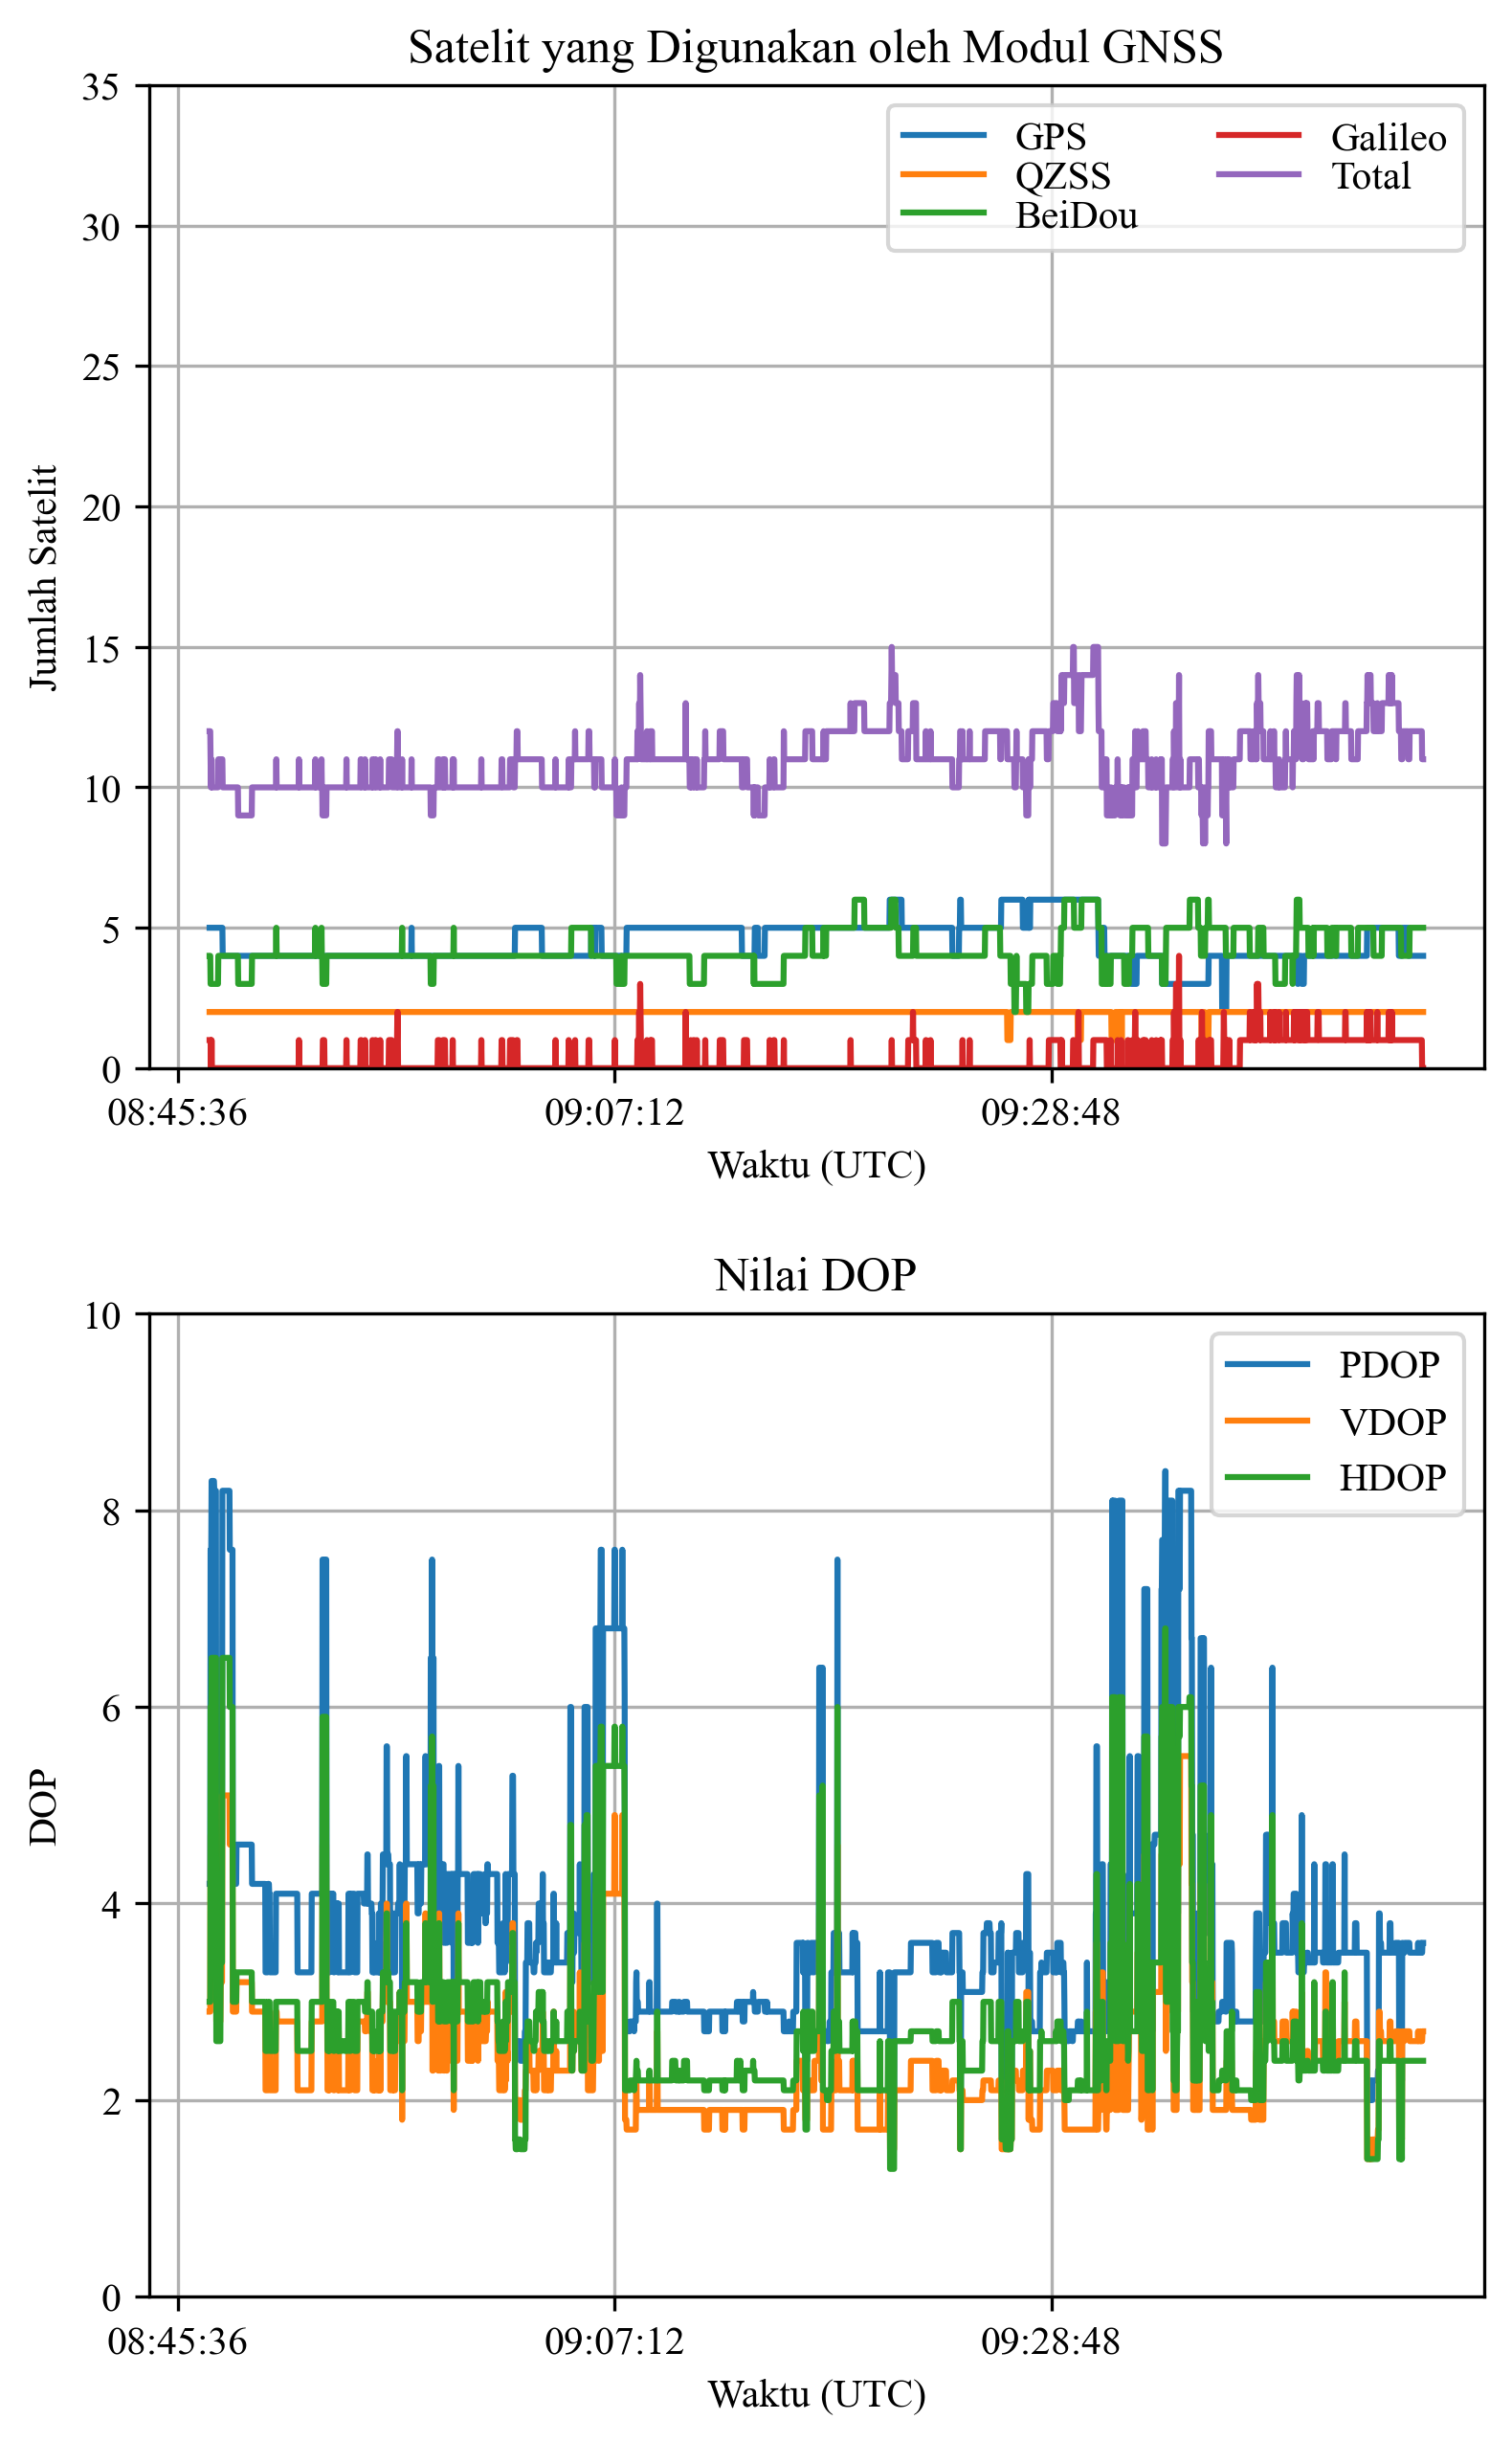
\includegraphics[width=12cm]{contents/chapter-4/2-skenario-indoor/sats_dop.png}
	\caption{Jumlah Satelit dan Nilai DOP pada Pengujian Skenario Dalam Ruangan Tertutup}
	\label{Fig: indoor-sats_dop}
\end{figure}

Nilai DOP yang lebih rendah menunjukan bahwa akurasi pada skenario ini lebih baik jika dibandingkan dengan skenario sebelumnya. Rata-rata nilai PDOP pada skenario ini adalah 3,73. Hal tersebut juga bersamaan dengan cakupan satelit yang lebih memenuhi lingkaran seperti ditunjukan oleh Gambar \ref{Fig: indoor-sky_plot}.

\begin{figure}[H]
	\centering
	\captionsetup{justification=centering}
	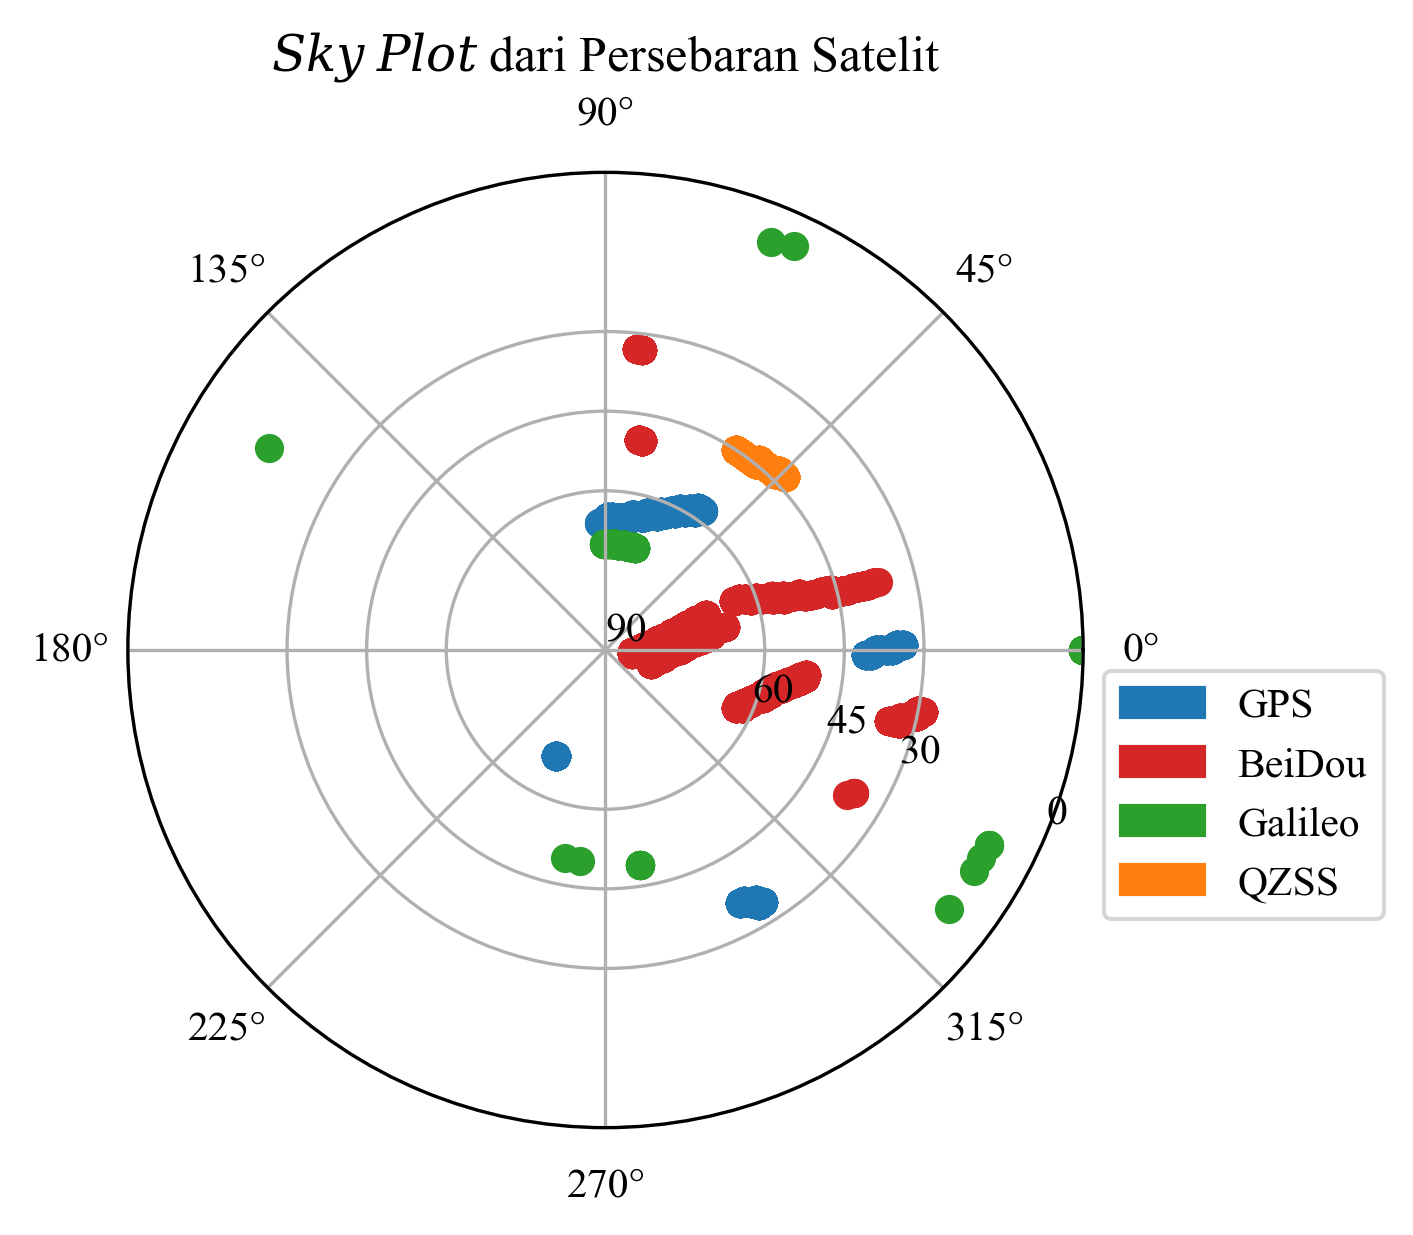
\includegraphics[width=12cm]{contents/chapter-4/2-skenario-indoor/sky_plot.png}
	\caption{\textit{Sky Plot} Skenario Dalam Ruangan}
	\label{Fig: indoor-sky_plot}
\end{figure}

Rata-rata CEP pada skenario dalam ruangan adalah 12,14 m atau 37,14\% lebih presisi jika dibandingkan dengan skenario \textit{basement}. Tabel \ref{Tab: indoor-table} menunjukan bahwa rata-rata nilai HDOP pada pengujian ini adalah 2,79 yang menunjukan bahwa hasil pengukuran sudah baik dan tepat berada pada standar minimum pengukuran. Struktur beton yang lebih sedikit dapat membantu untuk meningkatkan performa GNSS terlihat pada semakin banyak satelit yang dapat digunakan dan penurunan pada nilai CEP dan ketiga nilai DOP.

\subsection{Skenario Ruangan Semi Terbuka}
\begin{table}[H]
	\caption{Jenis STM32 dan Arsitekturnya}
	\vspace{0.5em}
	\centering
	\begin{tabular}{ccccc}
		\hline
		& \textbf{Minima} & \textbf{Maxima} & \textbf{Rata-rata} & \textbf{Standar Deviasi}\\
		\hline 
		HDOP & 1,30	& 6,80 & 2,79 & 0,96\\
		PDOP & 1,40	& 5,50 & 2,48 & 0,79\\
		VDOP & 2,00	& 8,40 & 3,73 & 1,22\\
		CEP & 9,51	& 33,27 & 12,14 & 4,02\\
		Jumlah Satelit & 8 & 15 & 10,93 & 1,14\\
		\hline
	\end{tabular}
	\label{Tab: semioutdoor-table}
\end{table}

\subsection{Skenario Luar Ruangan}
\begin{table}[H]
	\caption{Jenis STM32 dan Arsitekturnya}
	\vspace{0.5em}
	\centering
	\begin{tabular}{ccccc}
		\hline
		& \textbf{Minima} & \textbf{Maxima} & \textbf{Rata-rata} & \textbf{Standar Deviasi}\\
		\hline 
		HDOP & 0,60 & 0,80 & 0,65 & 0,06 \\
		PDOP & 0,90 & 1,60 & 1,12 & 0,15 \\
		VDOP & 1,10	& 1,80 & 1,30 & 0,15 \\
		CEP & 5,22 & 6,80 & 6,12 & 0,41 \\
		Jumlah Satelit & 17	& 25 & 21,14 & 1,37 \\
		\hline
	\end{tabular}
	\label{Tab: outdoor-table}
\end{table}

\section{Pengujian di Bus Trans Gadjah Mada}